\documentclass{beamer}
\title[Freedom~101] {Freedom to Teach}
\subtitle{\href{https://bringittogether.ca}{@BIT16}}
\author{Marc~Lijour}
\date{November~10, 2016}
\subject{Privacy and Security meet Freedom}
\usepackage{tikz}
%
\logo{
\includegraphics[scale=.1]{./images/logo-sfl-250.png}}
\AtBeginSection[]
{
  \begin{frame}
    \frametitle{Table of Contents}
    \tableofcontents[currentsection]
  \end{frame}
}
\usetheme{Boadilla}
%\usepackage[format=plain,justification=raggedright,singlelinecheck=false]{caption}
\usepackage[format=plain,justification=justified,singlelinecheck=false]{caption}
\usepackage[utf8]{inputenc}
\usepackage{dirtytalk}
\usepackage{wrapfig}
%\usepackage[pdfauthor={Marc Lijour},pdftitle={Freedom to Teach},pagebackref=true]{hyperref}
\usepackage{hyperref}
\usepackage{verbatim}
\usepackage{mathabx}
%\usepackage{MnSymbol}
\usepackage{outlines}
% To make underlined links
%http://tex.stackexchange.com/questions/26071/how-can-i-have-colored-and-underlined-links-with-hyperref
%\hypersetup{%
%  colorlinks=true,% hyperlinks will be coloured
%  linkcolor=blue,% hyperlink text will be green
%  linkbordercolor=purple,% hyperlink border will be red
%}
%\makeatletter
%\Hy@AtBeginDocument{%
%  \def\@pdfborder{0 0 1}% Overrides border definition set with colorlinks=true
%  \def\@pdfborderstyle{/S/U/W 1}% Overrides border style set with colorlinks=true
%                                % Hyperlink border style will be underline of width 1pt
%}
%\makeatother

\begin{document}
\frame{
%	\tikz[remember picture,overlay]
%	  \node at
%		([xshift=2cm,yshift=2cm]current page.south west)
%		%([xshift=10.5cm,yshift=-3cm]current page.west)
%		{
\includegraphics[width=3cm,height=3cm]{./images/logo-sfl-250.png}};
	\titlepage
}

\begin{frame}
\frametitle{Table of Contents}
\tableofcontents[currentsection]
\end{frame}

%%%%%%%%%%%%%% 1st SECTION: Intro %%%%%%%%%%%%%%%%%
\section[Section]{Introductions}
	\begin{frame}
	\frametitle{Presenter: Marc Lijour}
	\framesubtitle{Helping businesses and countries digitize}
	\tikz[remember picture,overlay]
	  \node at
		([xshift=-2.1cm,yshift=-1.5cm]current page.north east)
		{
\includegraphics[width=3cm,height=3cm]{./images/logo-sfl-250.png}};
	%Content goes here
	%\emph{Helping businesses and countries digitize}
	%\vspace{1.2cm}
		\begin{itemize}
			\item Director @ Savoir-faire Linux
			\item OCT, Maths, Computer Science
			\item Former Education Officer @Ministry of Education\\{\tiny{(Tech Ed \& Computer Studies Curriculum, e-Learning Ontario)}}
			\item Using Free Software since 1999
			\item Non-profit: Officer of the ICTC Board, PIEneer with Prepr Foundation
		\end{itemize}
	\end{frame}

%%%%%%%%%%%%%% 2nd SECTION: State of Tech & Teaching Today %%%%%%%%%%%%%%%%%
\section[Section]{Teaching with technology in 2016}
	\begin{frame}
	\frametitle{Teaching \& Technology}
	\framesubtitle{}
	        \begin{figure}[h]
                \centering
                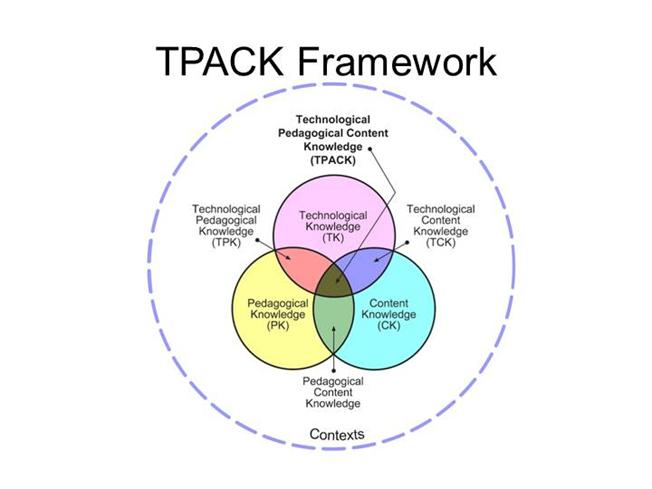
\includegraphics[width=.8\textwidth]{./images/tpack2}
		\caption{from \href{https://www.commonsensemedia.org/videos/introduction-to-the-tpack-model}{Common sense media}}
        	\end{figure}
	\end{frame}

	\begin{frame}
	\frametitle{Karen Billing's take on EdTech}
	\framesubtitle{}
	        \begin{figure}[h]
                \centering
                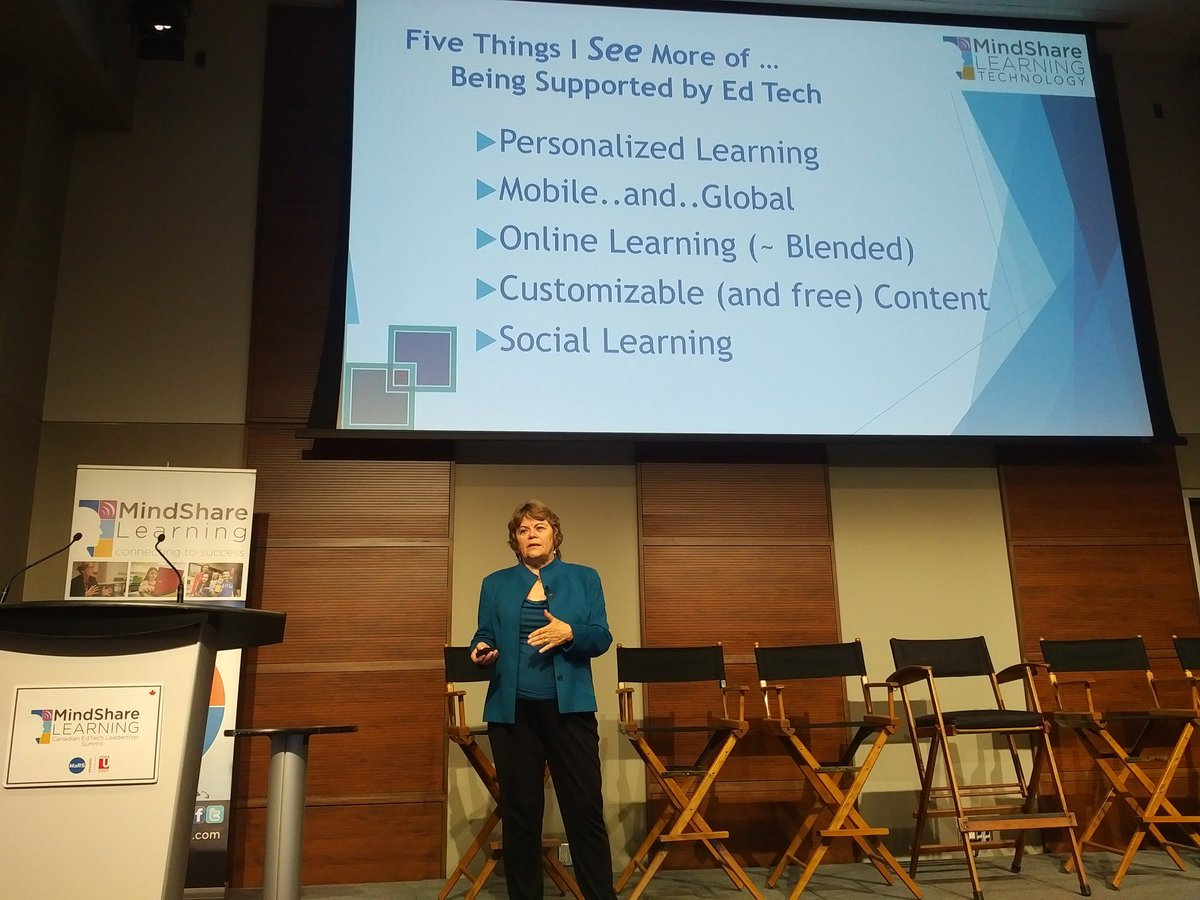
\includegraphics[width=.8\textwidth]{./images/KarenBillings-5thingsmore}
		\caption{Credit @ Robert Martellacci (\href{https://twitter.com/MindShareLearn/status/794166169477545984}{on Twitter})}
        	\end{figure}
	\end{frame}

	\begin{frame}
	\frametitle{A slow motion digitization of learning}
	\framesubtitle{}
		\begin{itemize}[<+->]
			\item 70's openness
			\item 80's personal computer
			\item 90's 'fat clients', software packages
			\item 00's web, web2.0
			\item 10's cloud-centric
			\item present: strengthening trend towards decentralization
		\end{itemize}
	\end{frame}

	\begin{frame}
	\frametitle{PC vs Mobile}
	\framesubtitle{}
	        \begin{figure}[h]
                \centering
                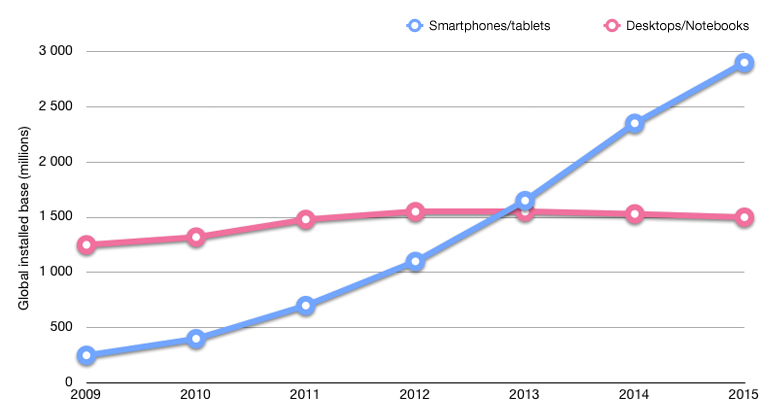
\includegraphics[width=.8\textwidth]{./images/mobile_vs_desktop}
		\caption{\url{http://kacao.fr/blog/}}
        	\end{figure}
	\end{frame}

	\begin{frame}
	\frametitle{PC vs Mobile}
	\framesubtitle{}
	        \begin{figure}[h]
                \centering
                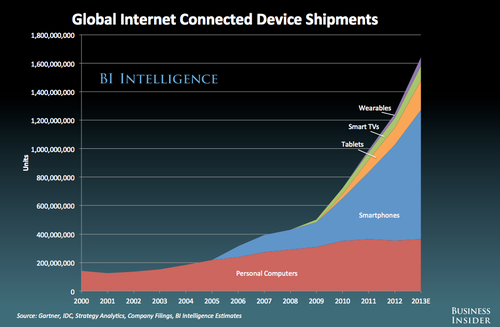
\includegraphics[width=.8\textwidth]{./images/globalIOTDeviceShipments}
		\caption{from \href{http://blog.kanyi.me/post/66994307568/contrarian-thinking-mobile-vs-pc-in-emerging}{Kanyi Maqubela's blog}}
        	\end{figure}
	\end{frame}

	\begin{frame}
	\frametitle{Microsoft's View on IoT by 2015}
	\framesubtitle{Azure + IoT}
	        \begin{figure}[h]
                \centering
                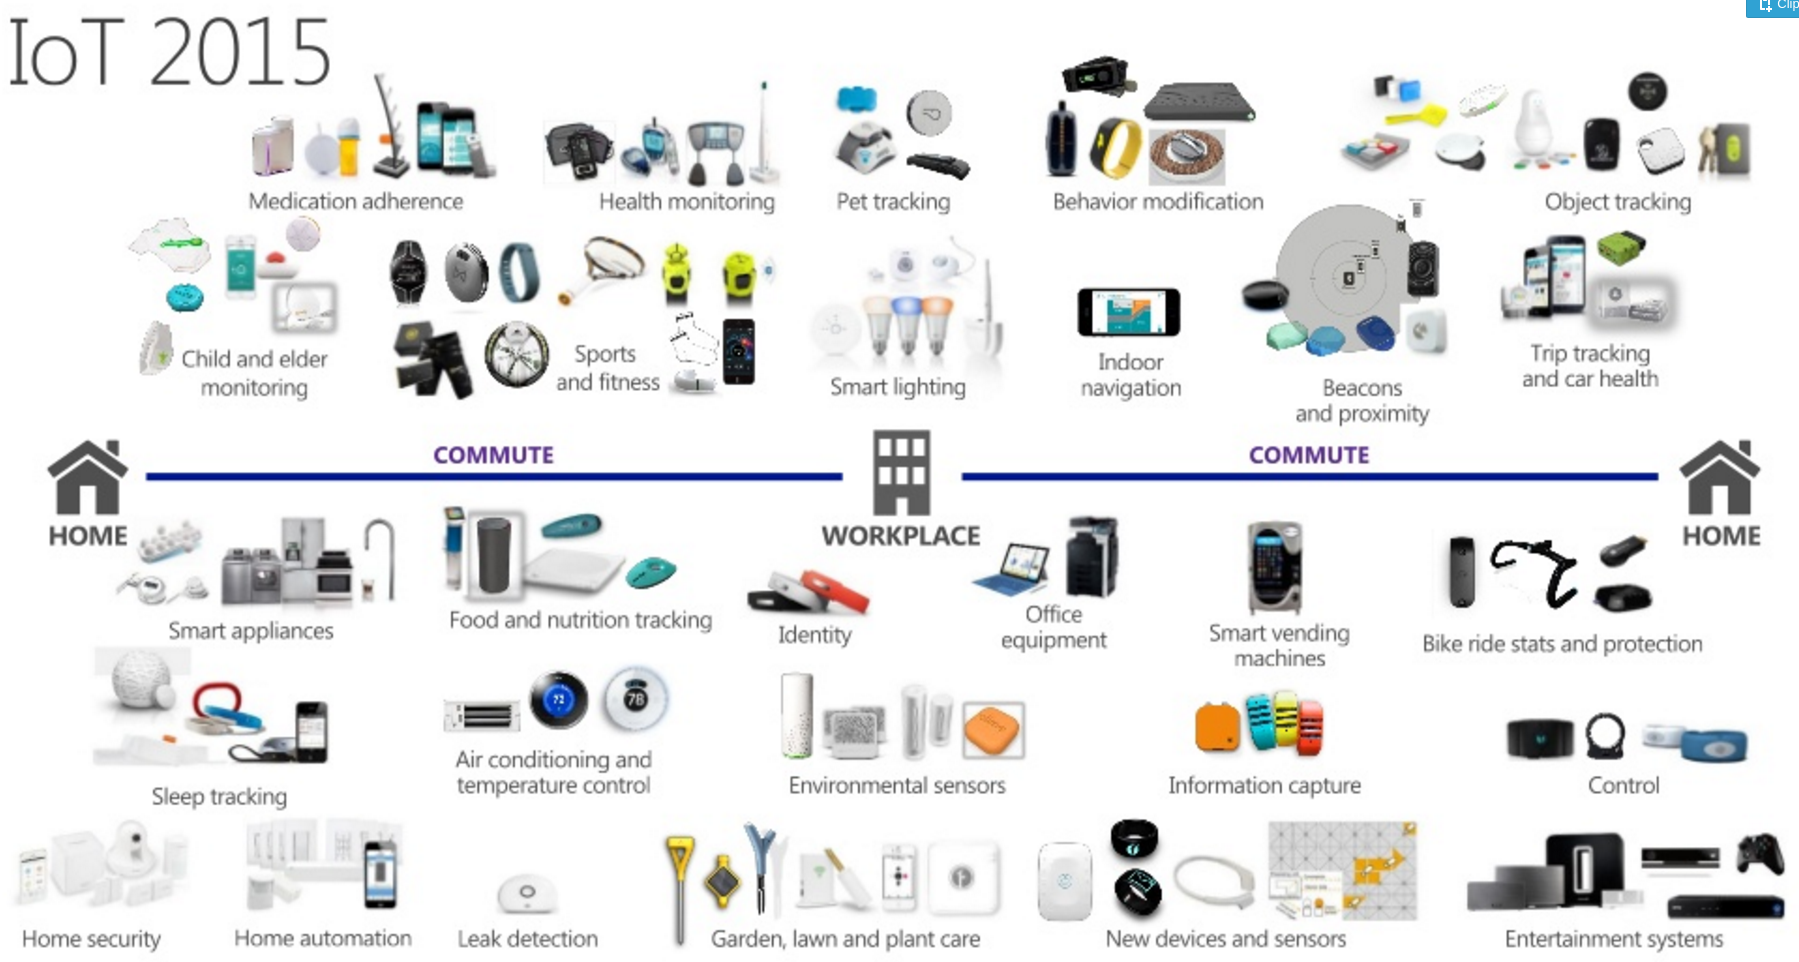
\includegraphics[width=.8\textwidth]{./images/msft-IoT2015}
		\caption{IoT across devices with Windows 10 and Azure IoT Suite by Admir Tuzović (on \href{http://www.slideshare.net/BosniaAgile/iot-across-devices-with-windows-10-and-azure-iot-suite-by-admir-tuzovi}{Slideshare})}
        	\end{figure}
	\end{frame}

	\begin{frame}
	\frametitle{All our data is online}
	\framesubtitle{}
	        \begin{figure}[h]
                \centering
                
\includegraphics[width=.8\textwidth]{./images/Cartoon_cloud.png}
        	\end{figure}
	\end{frame}


%%%%%%%%%%%%%% 3rd SECTION: The Case for Freedom %%%%%%%%%%%%%%%%%
\section[Section]{Challenges to our Freedom}
	\begin{frame}
	\frametitle{The meaning of Freedom}
	\framesubtitle{}
		\begin{itemize}[<+->]
			\item Do what you like while respecting the next in kind's freedom
			\item Democracy
			\item Citizenship
			\item Human Rights
			\item Rule of Law (Justice, Equity)
			\item Liberté - Égalité - Fraternité
		\end{itemize}
	\end{frame}

	\begin{frame}
	\frametitle{Freedom needs to be nurtured}
	\framesubtitle{}
	        \begin{figure}[h]
                \centering
                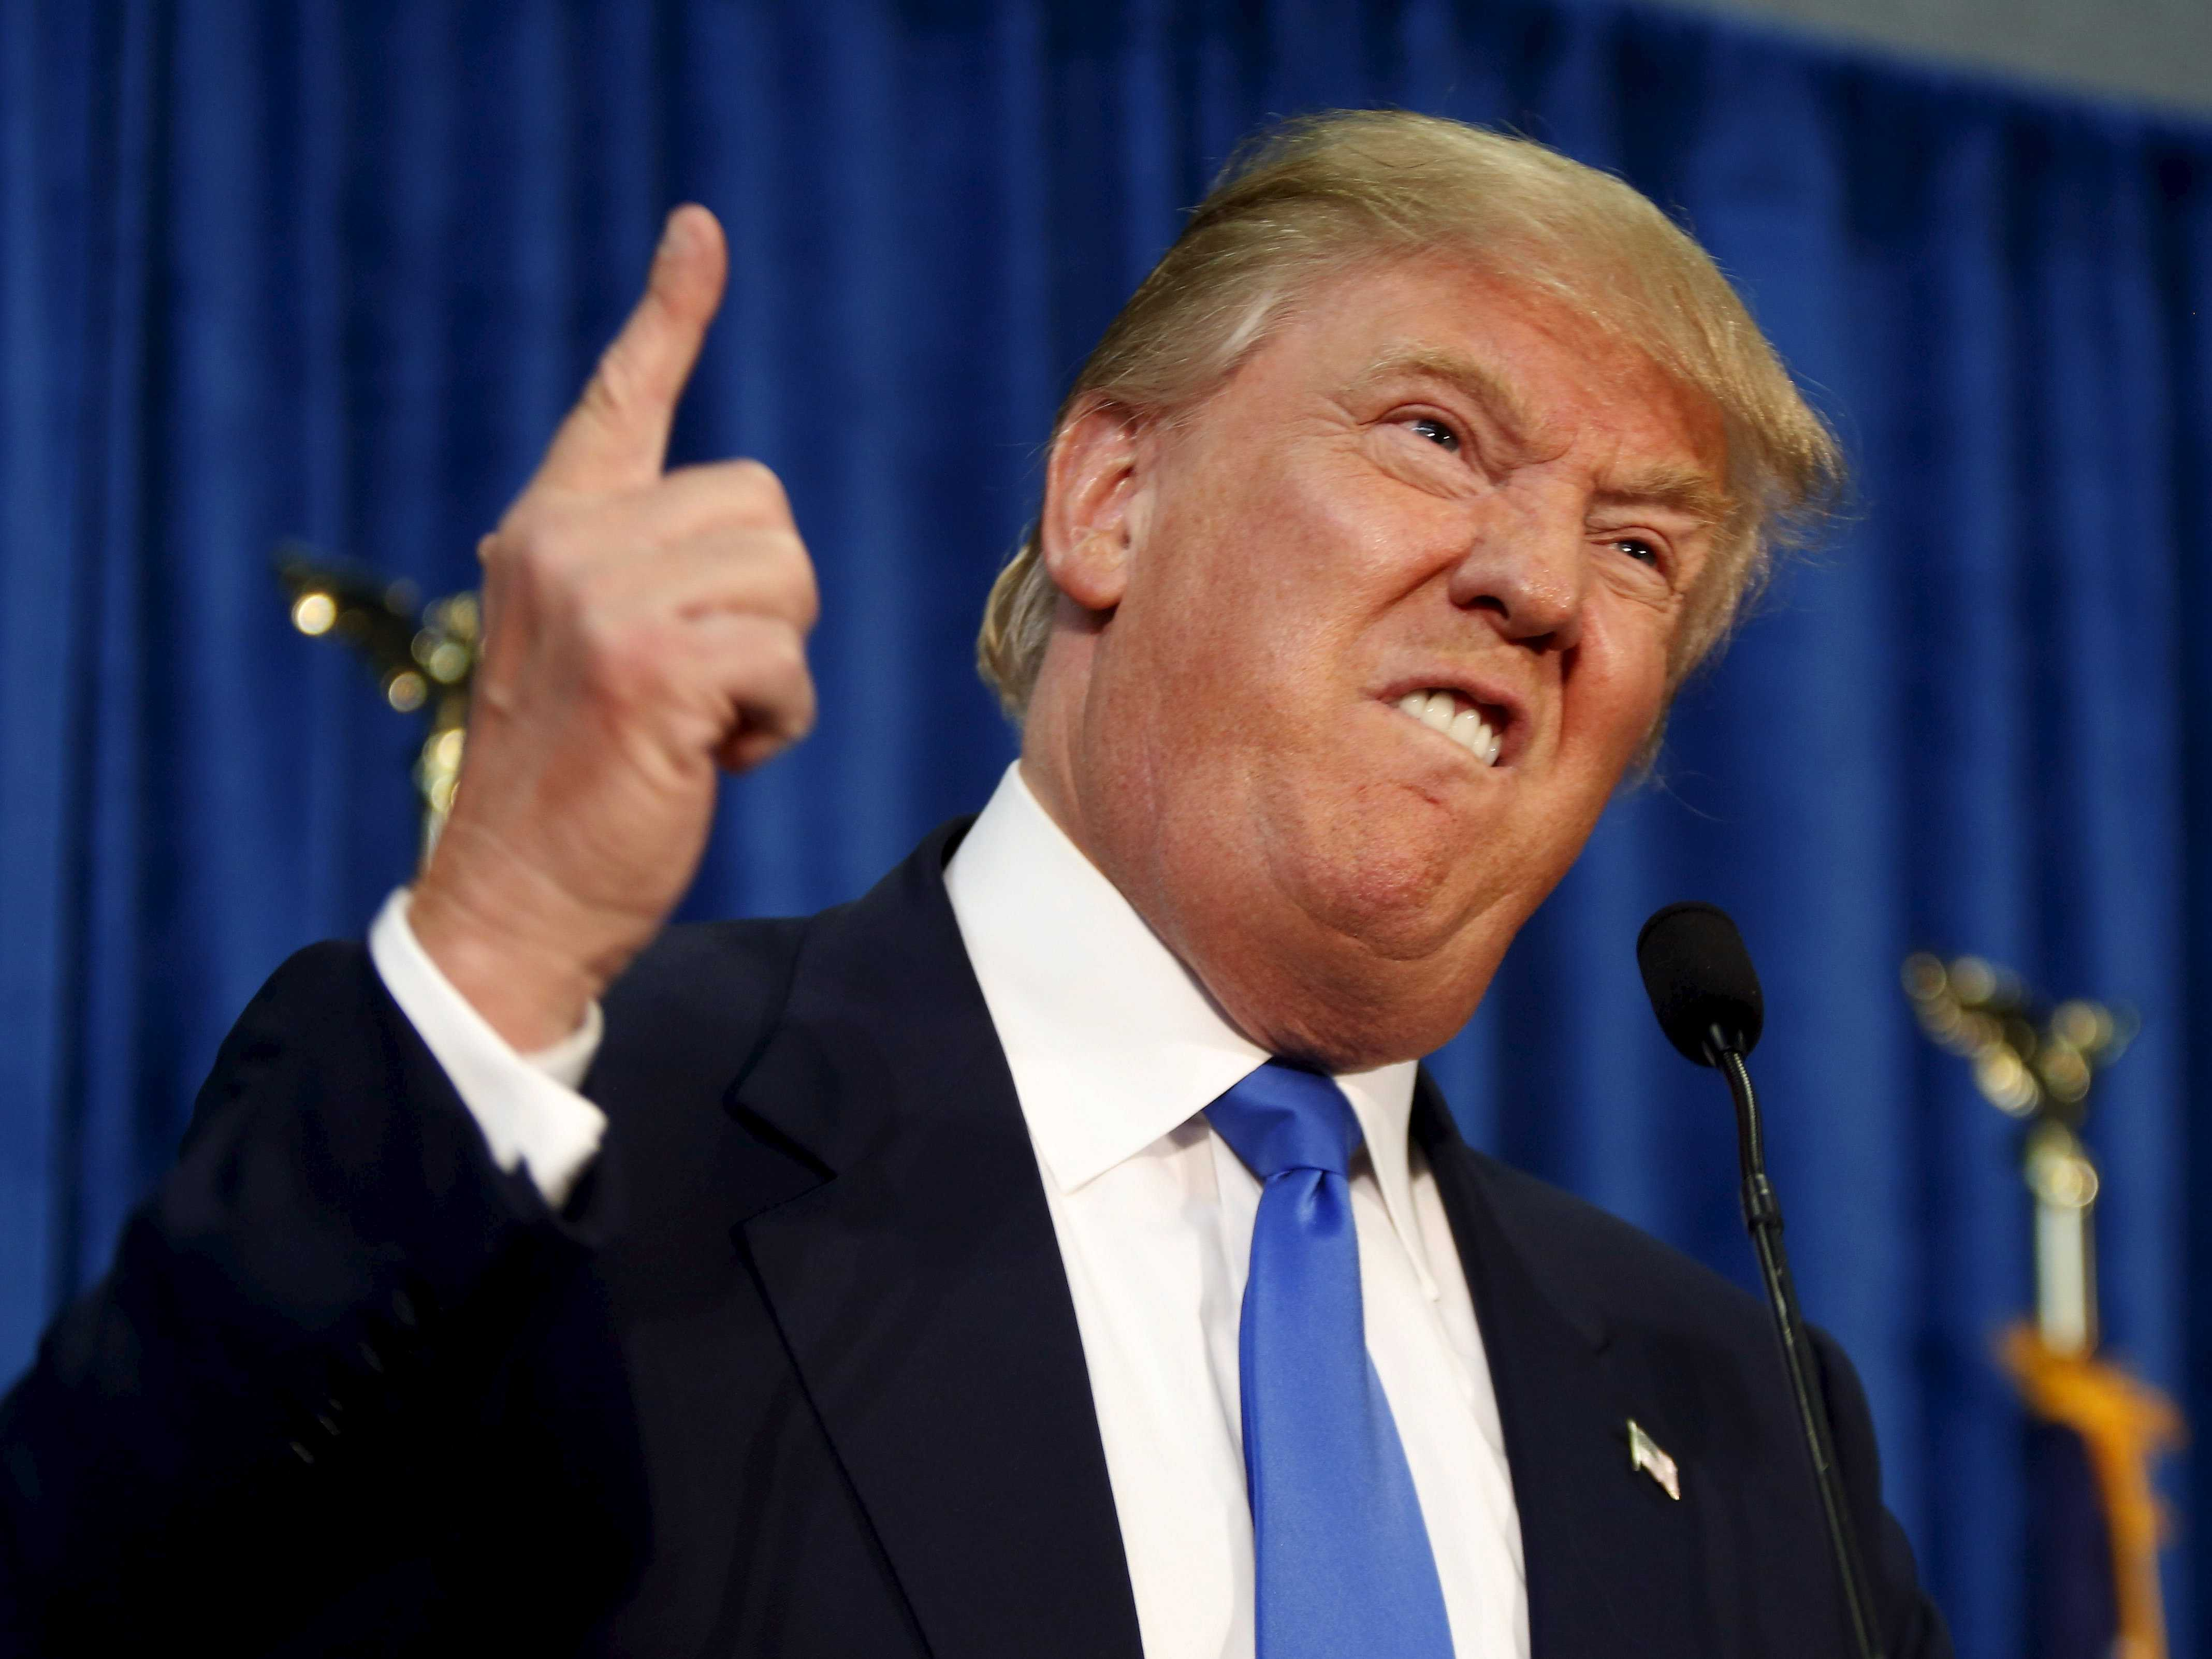
\includegraphics[width=.8\textwidth]{./images/Trump_fingerup}
		\caption{\tiny\url{http://www.zerohedge.com/news/2016-08-08/trump-financial-plan}}
        	\end{figure}
	\end{frame}

	\begin{frame}
	\frametitle{What could go wrong?}
	\framesubtitle{Excessive (?) Government Surveillance \& Intervention}
		\begin{itemize}[<+->]
			\item Citizen Biometric Registry (e.g. \href{http://www.pcworld.com/article/3139461/security/french-plan-for-biometric-database-of-60-million-people-sparks-outcry.html}{in France})
			\item Patriot Act (\& others: French Govnt Act, 2015...)
			\item Chinese Firewall
			\item Government-led Cyberattacks
		\end{itemize}
	\end{frame}

	\begin{frame}
	\frametitle{The User is the Product}
	\framesubtitle{GAFAM \& Corporate Interests under scrutiny}
		\begin{outline}
			\1 Google for example (see \href{http://www.forbes.com/sites/benkepes/2013/12/04/google-users-youre-the-product-not-the-customer/\#2871b0bc1624}{Forbes})
			\1 Microsoft \href{http://www.businessinsider.com/microsoft-shuts-down-scroogled-website-2015-1}{'Scroogled' Campaign} in reaction
			\1 In a case against Google, US Magistrate Judge Paul Grewal declared: "in this model, the users are the real product"
			\1 Follow the money:
				\2 US Internet Advertising Revenue in 2015: \$59.6 billion
				\2 Google: \$30 billion
				\2 Facebook: \$8 billion
			\1 Big Data \& Analytics is thriving with multiple data points (devices, apps, cameras...)
			\1 Organizations are vulnerable to security breaches
		\end{outline}
	\end{frame}


%%%%%%%%%%%%%% 4th SECTION: Solutions to saveguard Freedom %%%%%%%%%%%%%%%%%
\section[Section]{Working Efficiently AND (not OR) Protecting our Freedom}
	\begin{frame}
	\frametitle{Educate about Cybersecurity}
	\framesubtitle{Example: CyberTitan}
	\begin{columns}
		\column{0.5\textwidth}
			\begin{itemize}[<+->]
				\item ICTC program for high school students
				\item in partnership with the US Air Force Association’s CyberPatriot Program
				\item to develop in-demand skills needed to work in CyberSecurity, and other STEM areas
			\end{itemize}
		\column{0.5\textwidth}
	        	\begin{figure}[h]
                	\centering
                	
\includegraphics[width=.6\textwidth]{./images/CP_Cybertitan1-150x150}
			\caption{\url{http://www.cybertitan.ca}}
        		\end{figure}
	\end{columns}
	\end{frame}

	\begin{frame}
	\frametitle{Learn from Mozilla Internet Citizen}
	\framesubtitle{}
	        \begin{figure}[h]
                \centering
                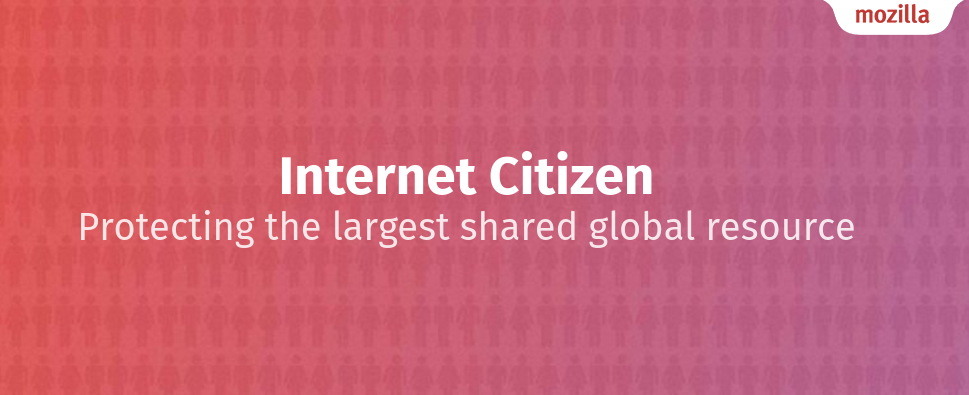
\includegraphics[width=.8\textwidth]{./images/moz-Internet-citizen}
		\caption{\url{https://blog.mozilla.org/internetcitizen/}}
        	\end{figure}
	\end{frame}

	\begin{frame}
	\frametitle{Solve the toughest 21st Century Challenges with PIE\tiny\textsuperscript{\textregistered}}
	\framesubtitle{}
	        \begin{figure}[h]
                \centering
                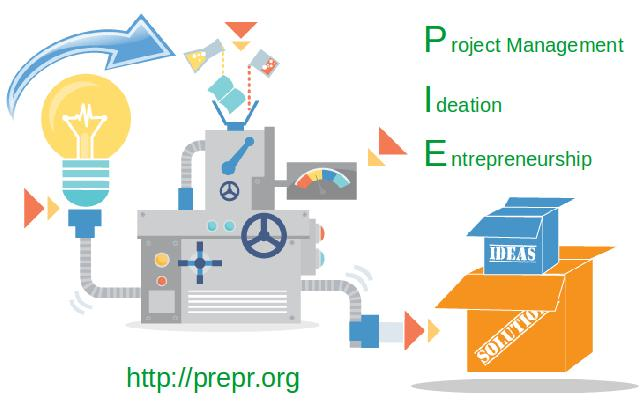
\includegraphics[width=.8\textwidth]{./images/PIE_slide}
		\caption{\url{https://prepr.org}}
        	\end{figure}
	\end{frame}

	\begin{frame}
	\frametitle{Design your EdTech Environment with Privacy in Mind}
	\framesubtitle{}
	       	\begin{figure}[h]
               	\centering
               	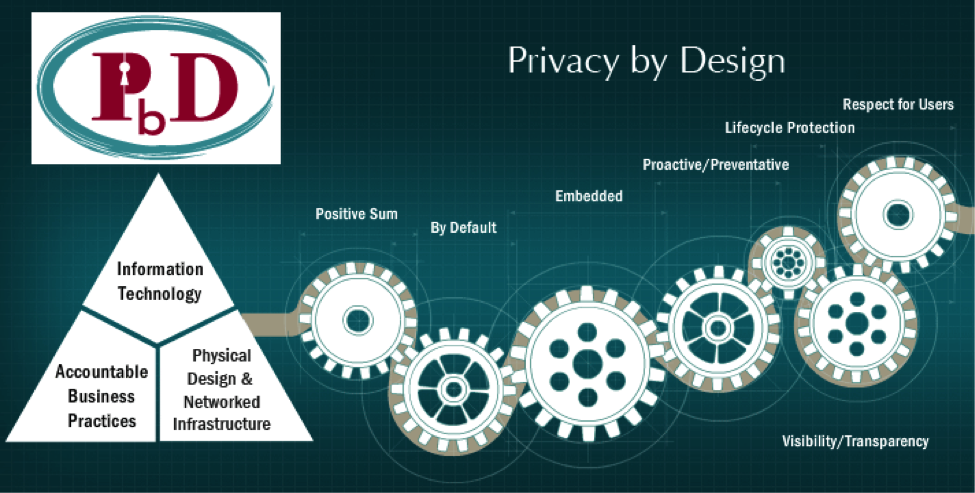
\includegraphics[width=.8\textwidth]{./images/privacybydesign}
		\caption{Dr. Ann Cavoukian, Executive Director, \href{http://www.ryerson.ca/pbdi/privacy-by-design/certification/TheSevenFoundationalPrinciplesofPrivacybyDesign/}{Privacy and Big Data Institute}}
        	\end{figure}
	\end{frame}

	\begin{frame}
	\frametitle{Prefer Decentralized Systems that put you in control}
	\framesubtitle{Examples: Blockchain, and Ring for Secure Communications}
	        \begin{figure}[h]
                \centering
                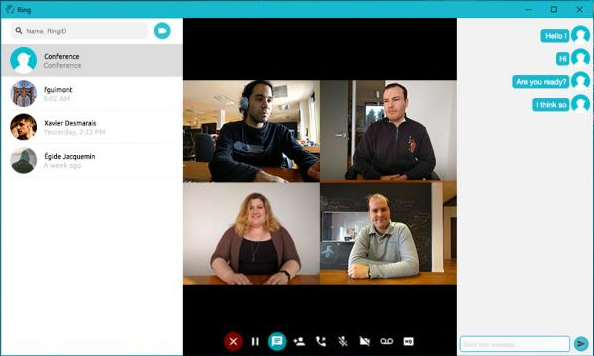
\includegraphics[width=.8\textwidth]{./images/ring_interface_desktop}
		\caption{Data is shared as a need-to-know basis, see \url{http://ring.cx}}
        	\end{figure}
	\end{frame}

	\begin{frame}
	\frametitle{Build Community Clouds that you control}
	\framesubtitle{}
		\begin{itemize}[<+->]
			\item Hosted in Canada
			\item On your premises or at a secure location
			\item As a school board, or an association of privacy-conscious teachers
			\item As an individual (for example on OVH or Microsoft Azure)
			\item With the help of students 
		\end{itemize}
	\end{frame}

	\begin{frame}
	\frametitle{Secure Clouds for your Pocket Book}
	\framesubtitle{OVH is the Top 3 Cloud Company with a data centre in Canada}
	        \begin{figure}[h]
                \centering
                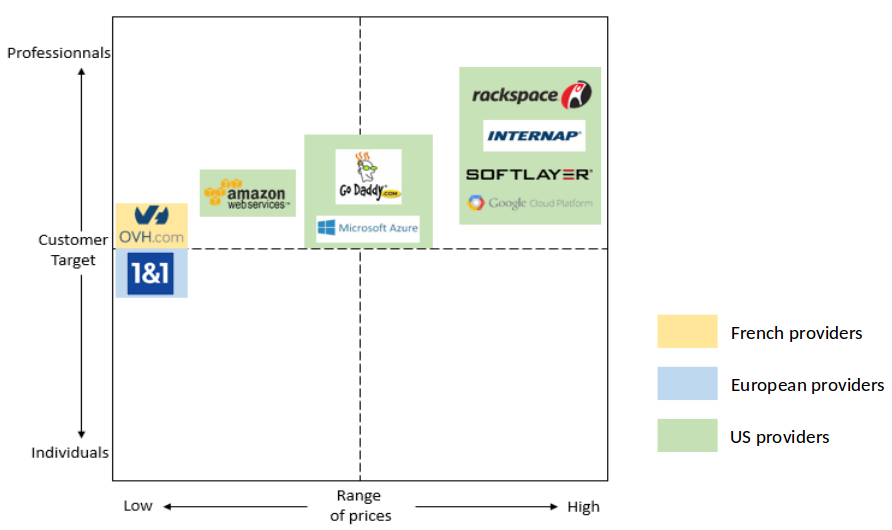
\includegraphics[width=.8\textwidth]{./images/OVH-cloud-magic-quadrant}
        	\end{figure}
	\end{frame}

	\begin{frame}
	\frametitle{OVH in Canada}
	\framesubtitle{}
		\begin{outline}
			\1 +30M\$ invested in Canada since 2013 
			\1 +3,000 Customers in Canada
			\1 2 PoP in Canada (Montreal and Toronto) and 11 in the US
			\1 Strategic partnerships:
				\2 Rogers as a reseller of Public Cloud Enterprise solutions Canada-wide 
				\2 VMWare (Partner Innovation Award received in 2016)
				\2 OpenStack (one of the 3 major contributors WW)
			\1 Technological partners: \textbf{Savoir-faire-Linux}, LinkByNet...%, S3 Technologies, Globalia…
%			\1 Hundreds of customers served in 40 countries (Middle East, Asia, LATAM, USA\ldots)
		\end{outline}
	        \begin{figure}[h]
                \centering
                
\includegraphics[width=.8\textwidth]{./images/OpenStack-Rogers-VMWare}
        	\end{figure}
	\end{frame}

	\begin{frame}
	\frametitle{OVH Global Footprint}
	\framesubtitle{\#1 in Europe, Top 3 Globally}
	        \begin{figure}[h]
                \centering
                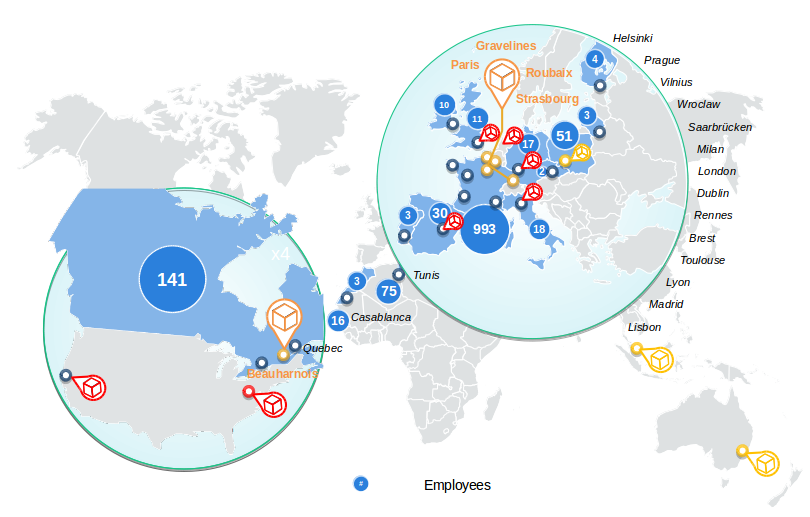
\includegraphics[width=.8\textwidth]{./images/OVH-global_presence}
        	\end{figure}
	\end{frame}

	\begin{frame}
	\frametitle{Build your own server / IoT device}
	\framesubtitle{with lunch money}
	        \begin{figure}[h]
                \centering
                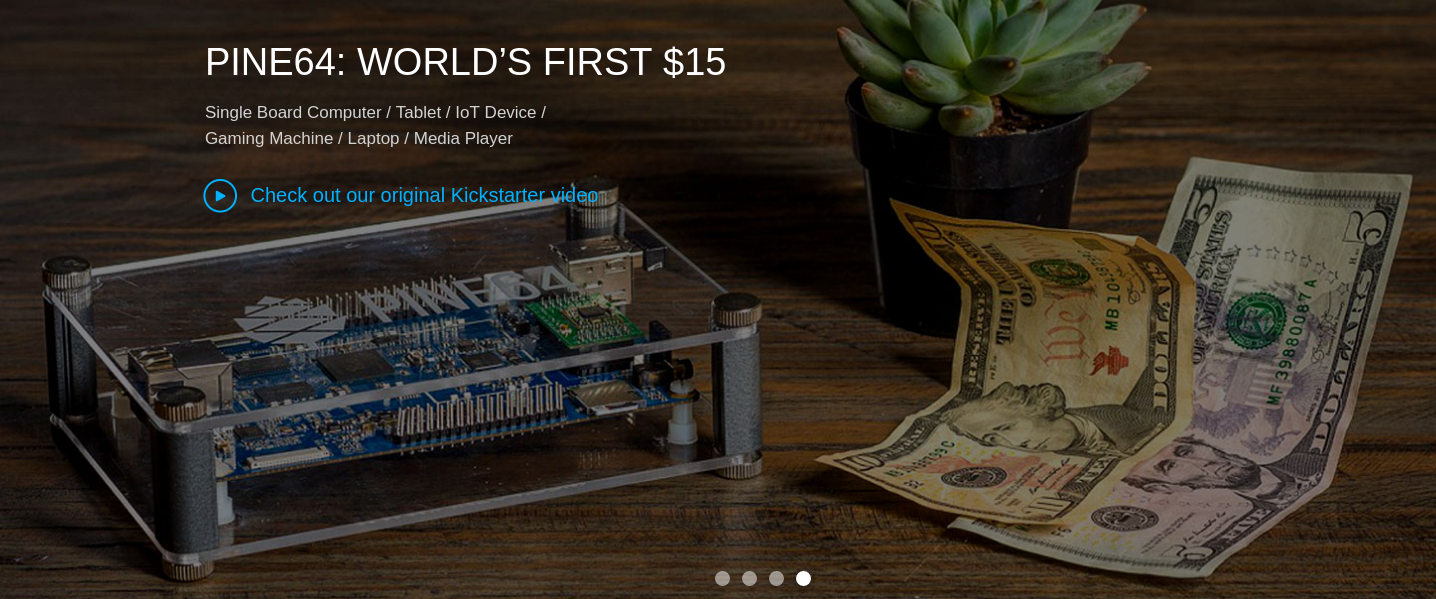
\includegraphics[width=.8\textwidth]{./images/pine64}
		\caption{\url{https://www.pine64.org}}
        	\end{figure}
	\end{frame}

	\begin{frame}
	\frametitle{Build your own server / IoT device}
	\framesubtitle{on a coffee budget}
	        \begin{figure}[h]
                \centering
                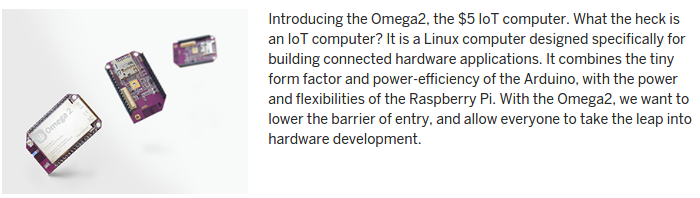
\includegraphics[width=.8\textwidth]{./images/Omega2}
		\caption{\tiny{\url{https://www.indiegogo.com/projects/omega2-5-linux-computer-with-wi-fi-made-for-iot}}}
        	\end{figure}
%		\url{https://www.indiegogo.com/projects/omega2-5-linux-computer-with-wi-fi-made-for-iot}
	\end{frame}

	\begin{frame}
	\frametitle{Use Free Software Alternatives}
	\framesubtitle{Example: Framasoft alternative to \href{https://blog.google/topics/education/introducing-g-suite-education/}{G Suite for Education} \& other popular SaaS}
	\begin{columns}
		\column{0.5\textwidth}
	        	\begin{figure}[h]
               		\centering
                	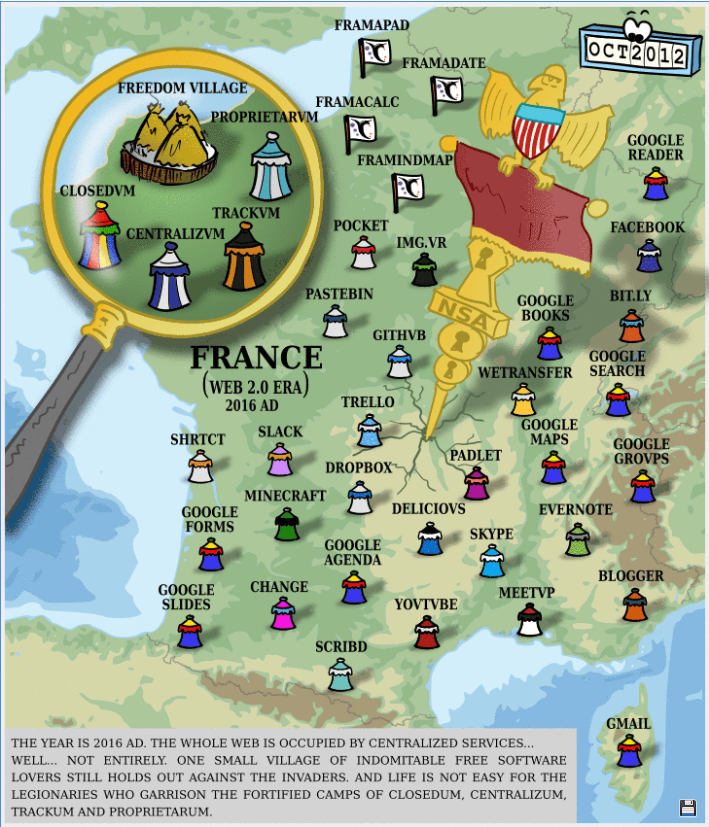
\includegraphics[width=.8\textwidth]{./images/framasoft-gaulle}
        		\end{figure}
		\column{0.5\textwidth}
	        	\begin{figure}[h]
                	\centering
                	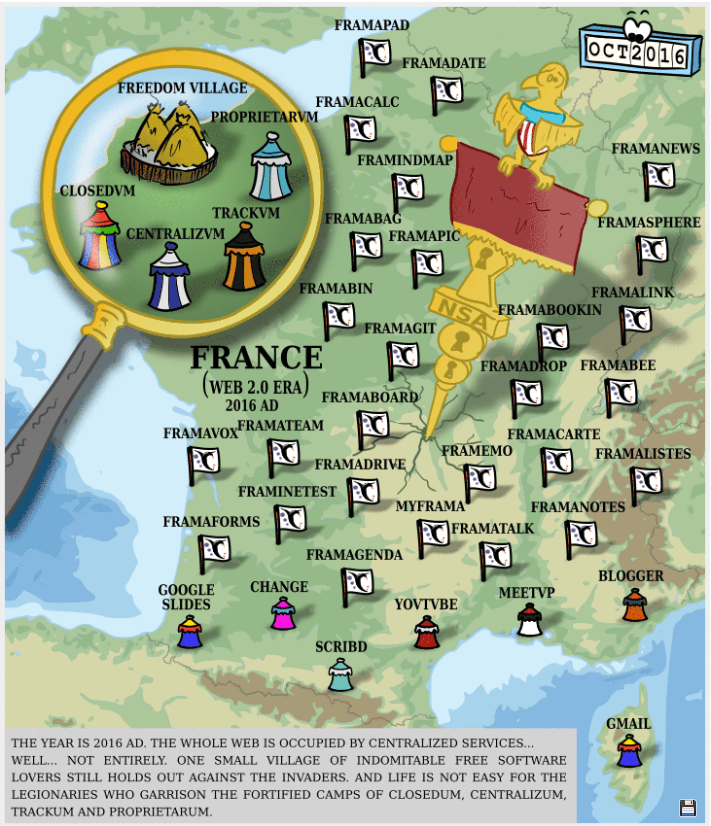
\includegraphics[width=.8\textwidth]{./images/framasoft-gaulle-201610}
        		\end{figure}
	\end{columns}
	\end{frame}

	\begin{frame}
	\frametitle{Framasoft}
	\framesubtitle{}
		\begin{itemize}
			\item Founded in France (2004)
			\item Promotes and educates about Free Software, Free Culture, Free Services
			\item Flagship project to offer Free/Libre alternatives to dominant proprietary offers
			\item 3 FTEs, and a large community
			\item 30 solutions online (SaaS), or download and install on your own cloud/server
		\end{itemize}
	\end{frame}

	\begin{frame}
	\frametitle{30 Framasoft Services}
	\framesubtitle{}
	        \begin{figure}[h]
                \centering
                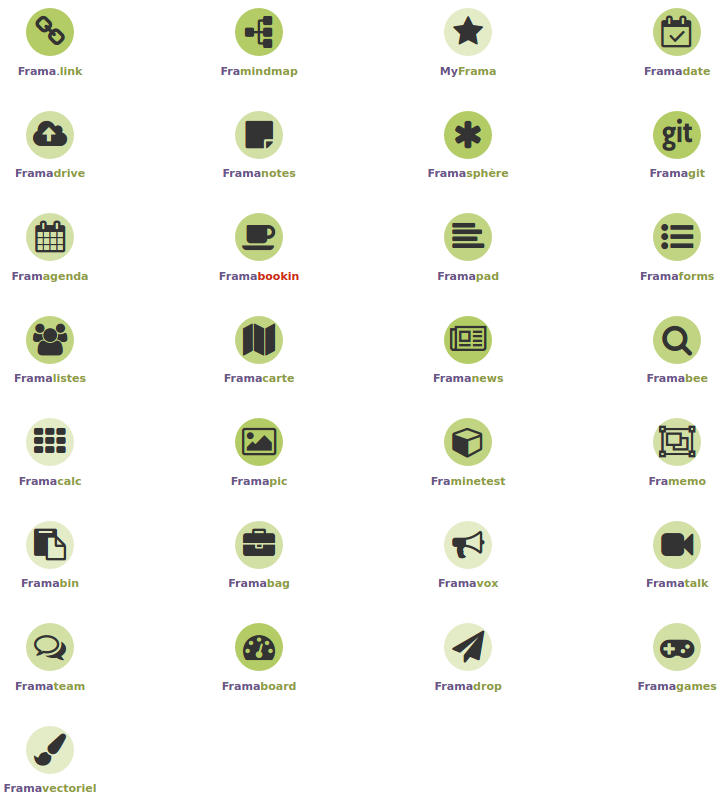
\includegraphics[width=.6\textwidth]{./images/framasoft-solutions}
        	\end{figure}
	\end{frame}

	\begin{frame}
	\frametitle{Framadrive $\leftrightarrow$ Google Drive}
	\framesubtitle{}
	        \begin{figure}[h]
                \centering
                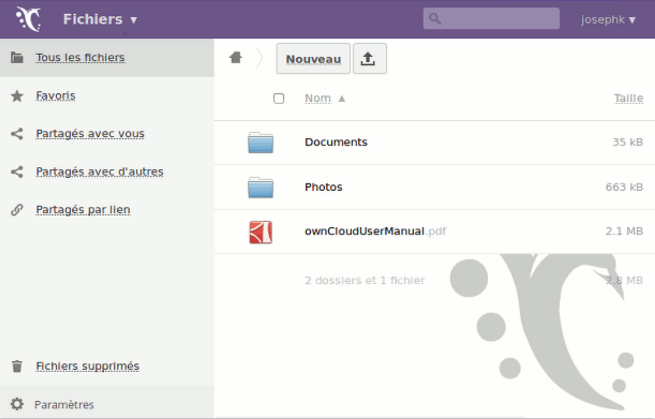
\includegraphics[width=.8\textwidth]{./images/framadrive}
		\caption{Based on \href{https://owncloud.org/}{OwnCloud} -with calendars, contacts, mobile app...}
        	\end{figure}
	\end{frame}

	\begin{frame}
	\frametitle{Framacalc $\leftrightarrow$ Google Spreadsheet}
	\framesubtitle{}
	        \begin{figure}[h]
                \centering
                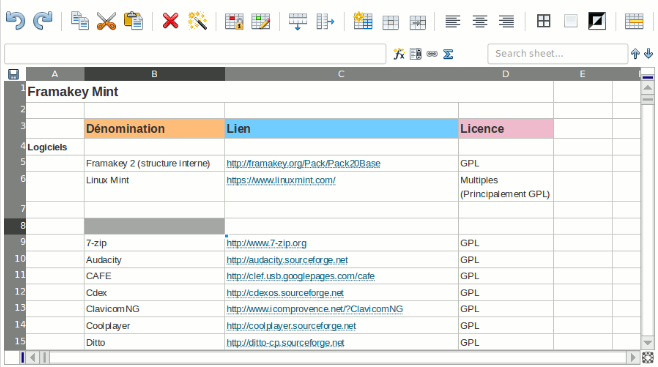
\includegraphics[width=.8\textwidth]{./images/framacalc}
		\caption{Based on \href{https://ethercalc.net}{EtherCalc}}
        	\end{figure}
	\end{frame}

	\begin{frame}
	\frametitle{Framagenda $\leftrightarrow$ Google Calendar}
	\framesubtitle{}
	        \begin{figure}[h]
                \centering
                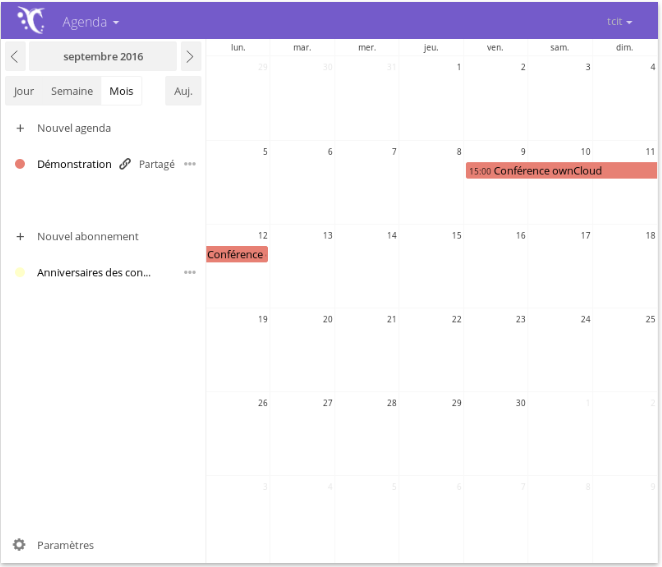
\includegraphics[width=.8\textwidth]{./images/framagenda}
		\caption{Based on \href{https://nextcloud.com}{NextCloud}}
        	\end{figure}
	\end{frame}

	\begin{frame}
	\frametitle{Framadate $\leftrightarrow$ Doodle}
	\framesubtitle{}
	        \begin{figure}[h]
                \centering
                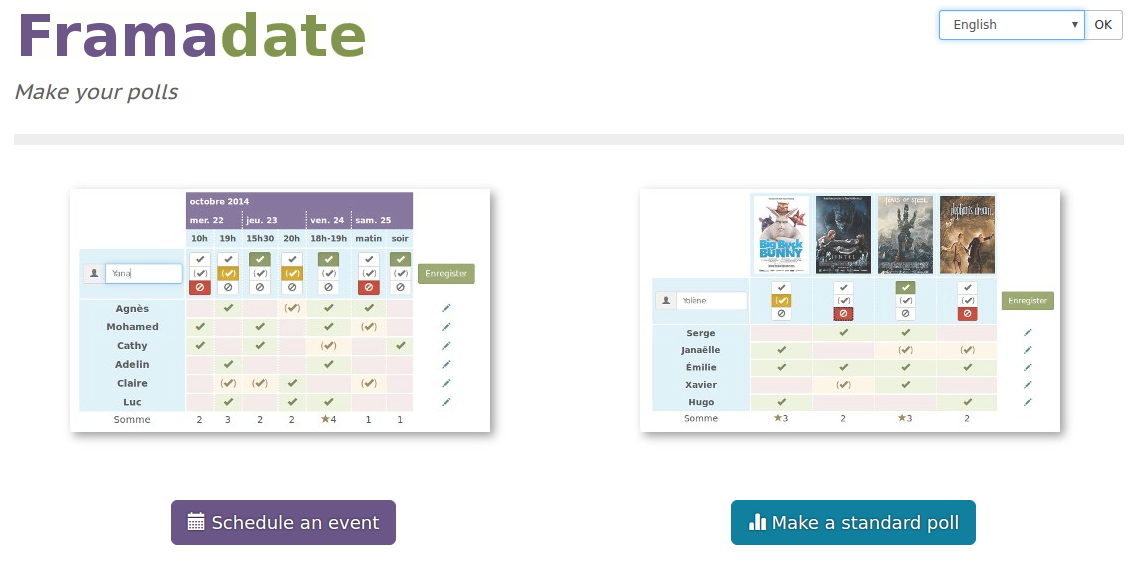
\includegraphics[width=.8\textwidth]{./images/framadate}
        	\end{figure}
	\end{frame}

	\begin{frame}
	\frametitle{Framapad $\leftrightarrow$ Evernote}
	\framesubtitle{}
	        \begin{figure}[h]
                \centering
                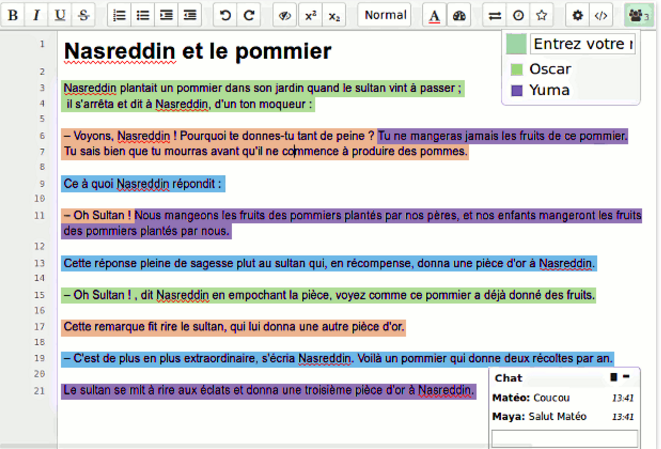
\includegraphics[width=.8\textwidth]{./images/framapad}
        	\end{figure}
	\end{frame}

	\begin{frame}
	\frametitle{Framacarte: Draw your own maps}
	\framesubtitle{}
	        \begin{figure}[h]
                \centering
                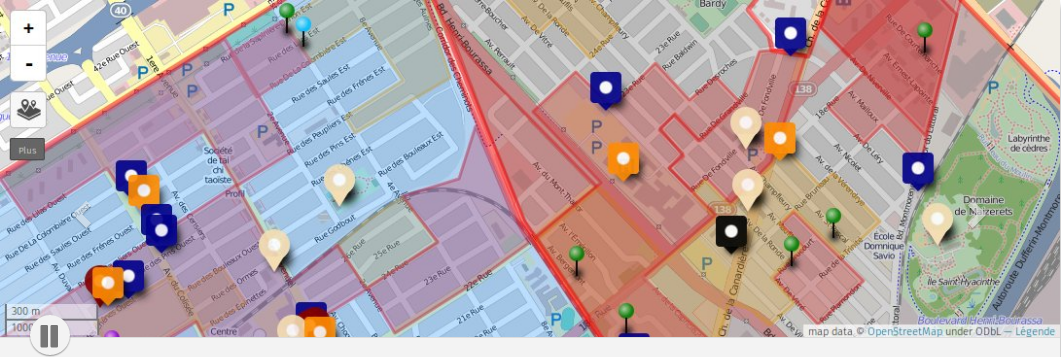
\includegraphics[width=.8\textwidth]{./images/framacarte}
		\caption{Based on \href{https://github.com/umap-project/umap/}{uMap} and \href{https://www.openstreetmap.org}{OpenStreetMap}} 
        	\end{figure}
	\end{frame}

	\begin{frame}
	\frametitle{Framinetest $\leftrightarrow$ Minecraft}
	\framesubtitle{}
	        \begin{figure}[h]
                \centering
                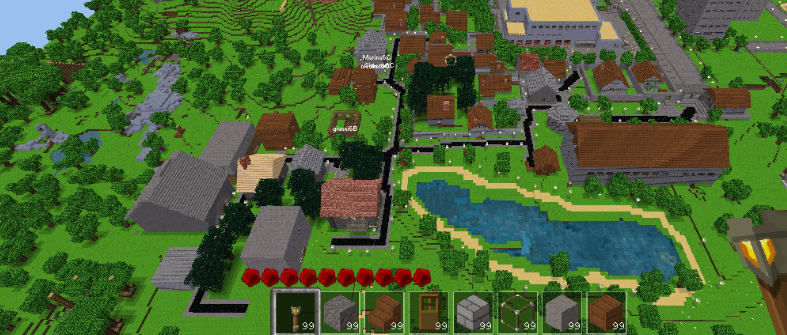
\includegraphics[width=.8\textwidth]{./images/framinetest}
		\caption{Based on \href{http://www.minetest.net}{Minetest}}
        	\end{figure}
	\end{frame}

	\begin{frame}
	\frametitle{Framamind $\leftrightarrow$ Inspiration / Freemind}
	\framesubtitle{}
	        \begin{figure}[h]
                \centering
                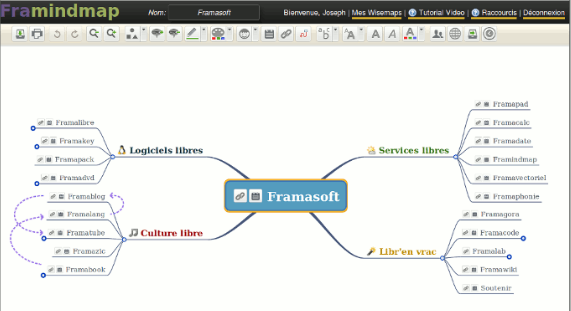
\includegraphics[width=.8\textwidth]{./images/framamind}
        	\end{figure}
	\end{frame}

	\begin{frame}
	\frametitle{Framabookin $\leftrightarrow$ Kindle Store (for free books)}
	\framesubtitle{}
	        \begin{figure}[h]
                \centering
                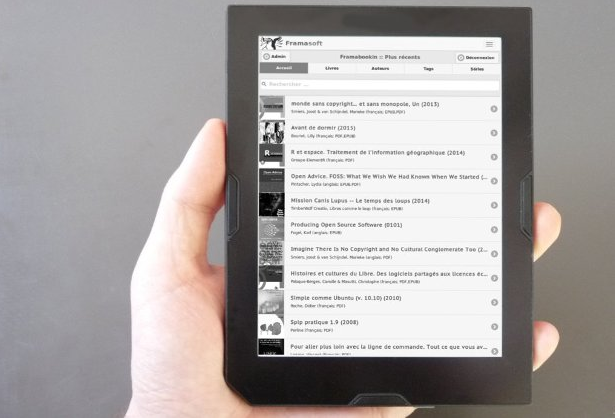
\includegraphics[width=.8\textwidth]{./images/framabookin}
        	\end{figure}
	\end{frame}

	\begin{frame}
	\frametitle{More Software -beyond Framasoft}
	\framesubtitle{}
	\begin{columns}
		\column{0.5\textwidth}
	        	\begin{figure}[h]
               		\centering
                	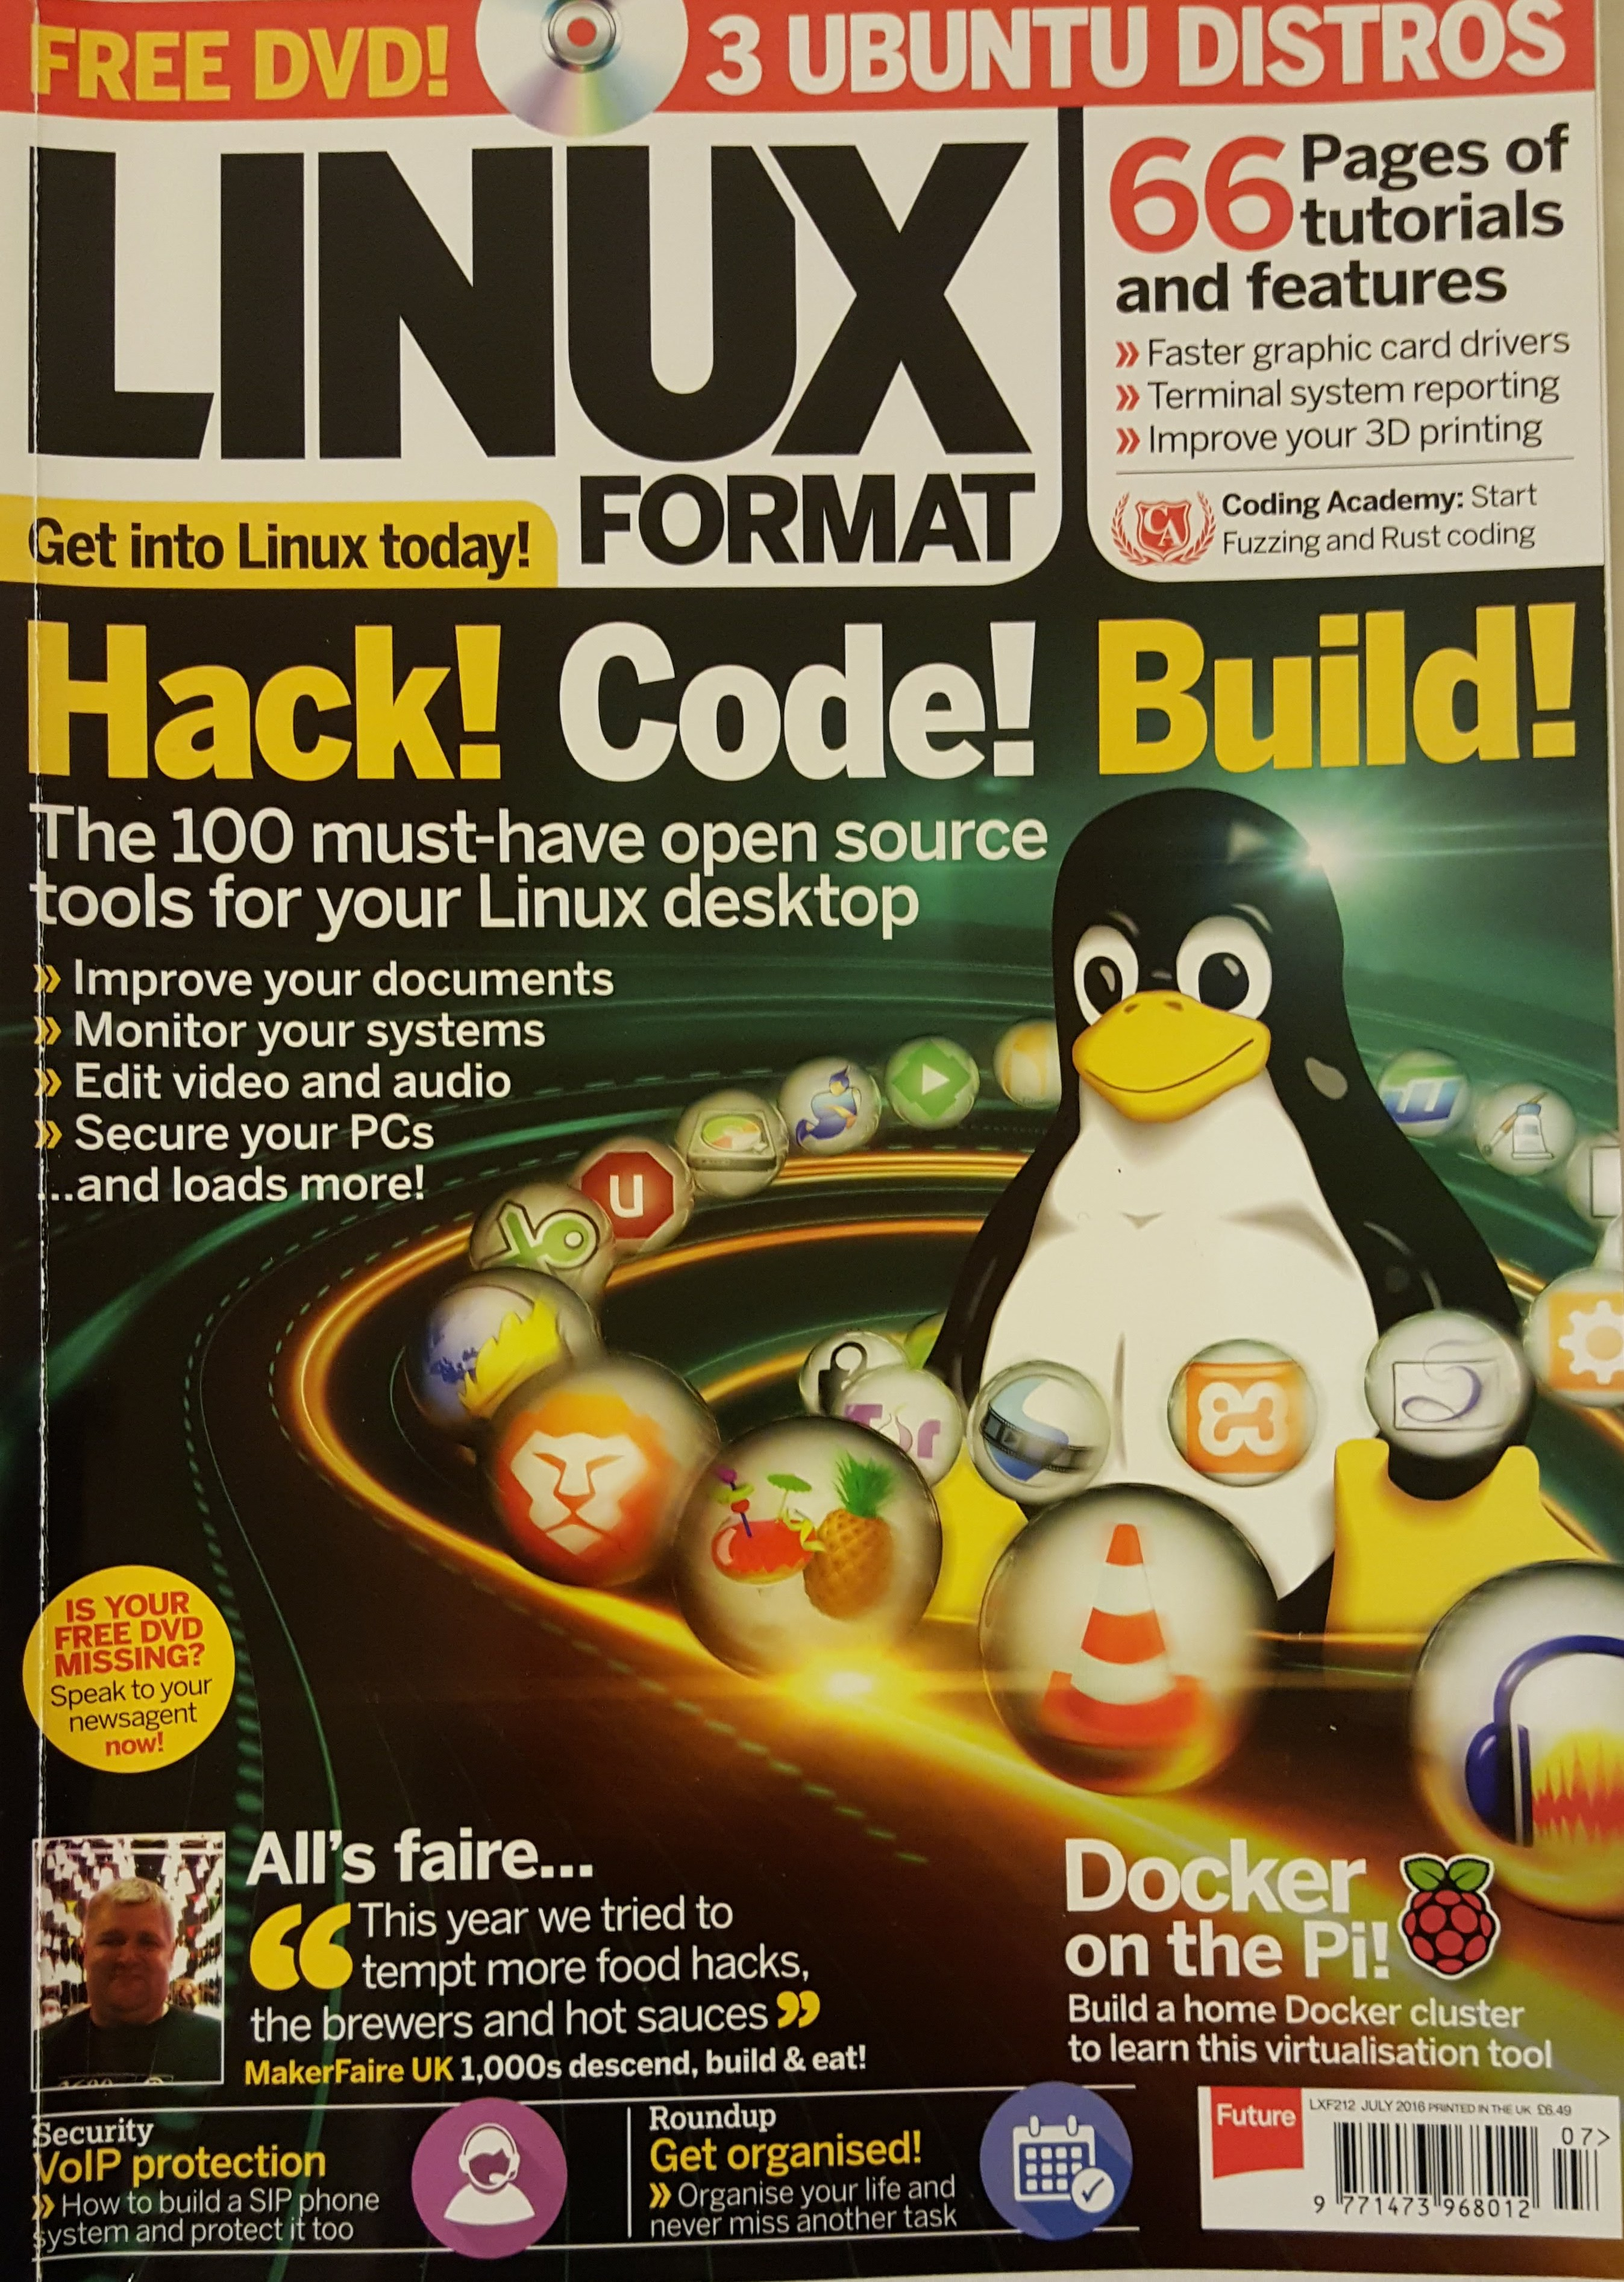
\includegraphics[width=.8\textwidth]{./images/LF-201607}
        		\end{figure}
		\column{0.5\textwidth}
	        	\begin{figure}[h]
                	\centering
                	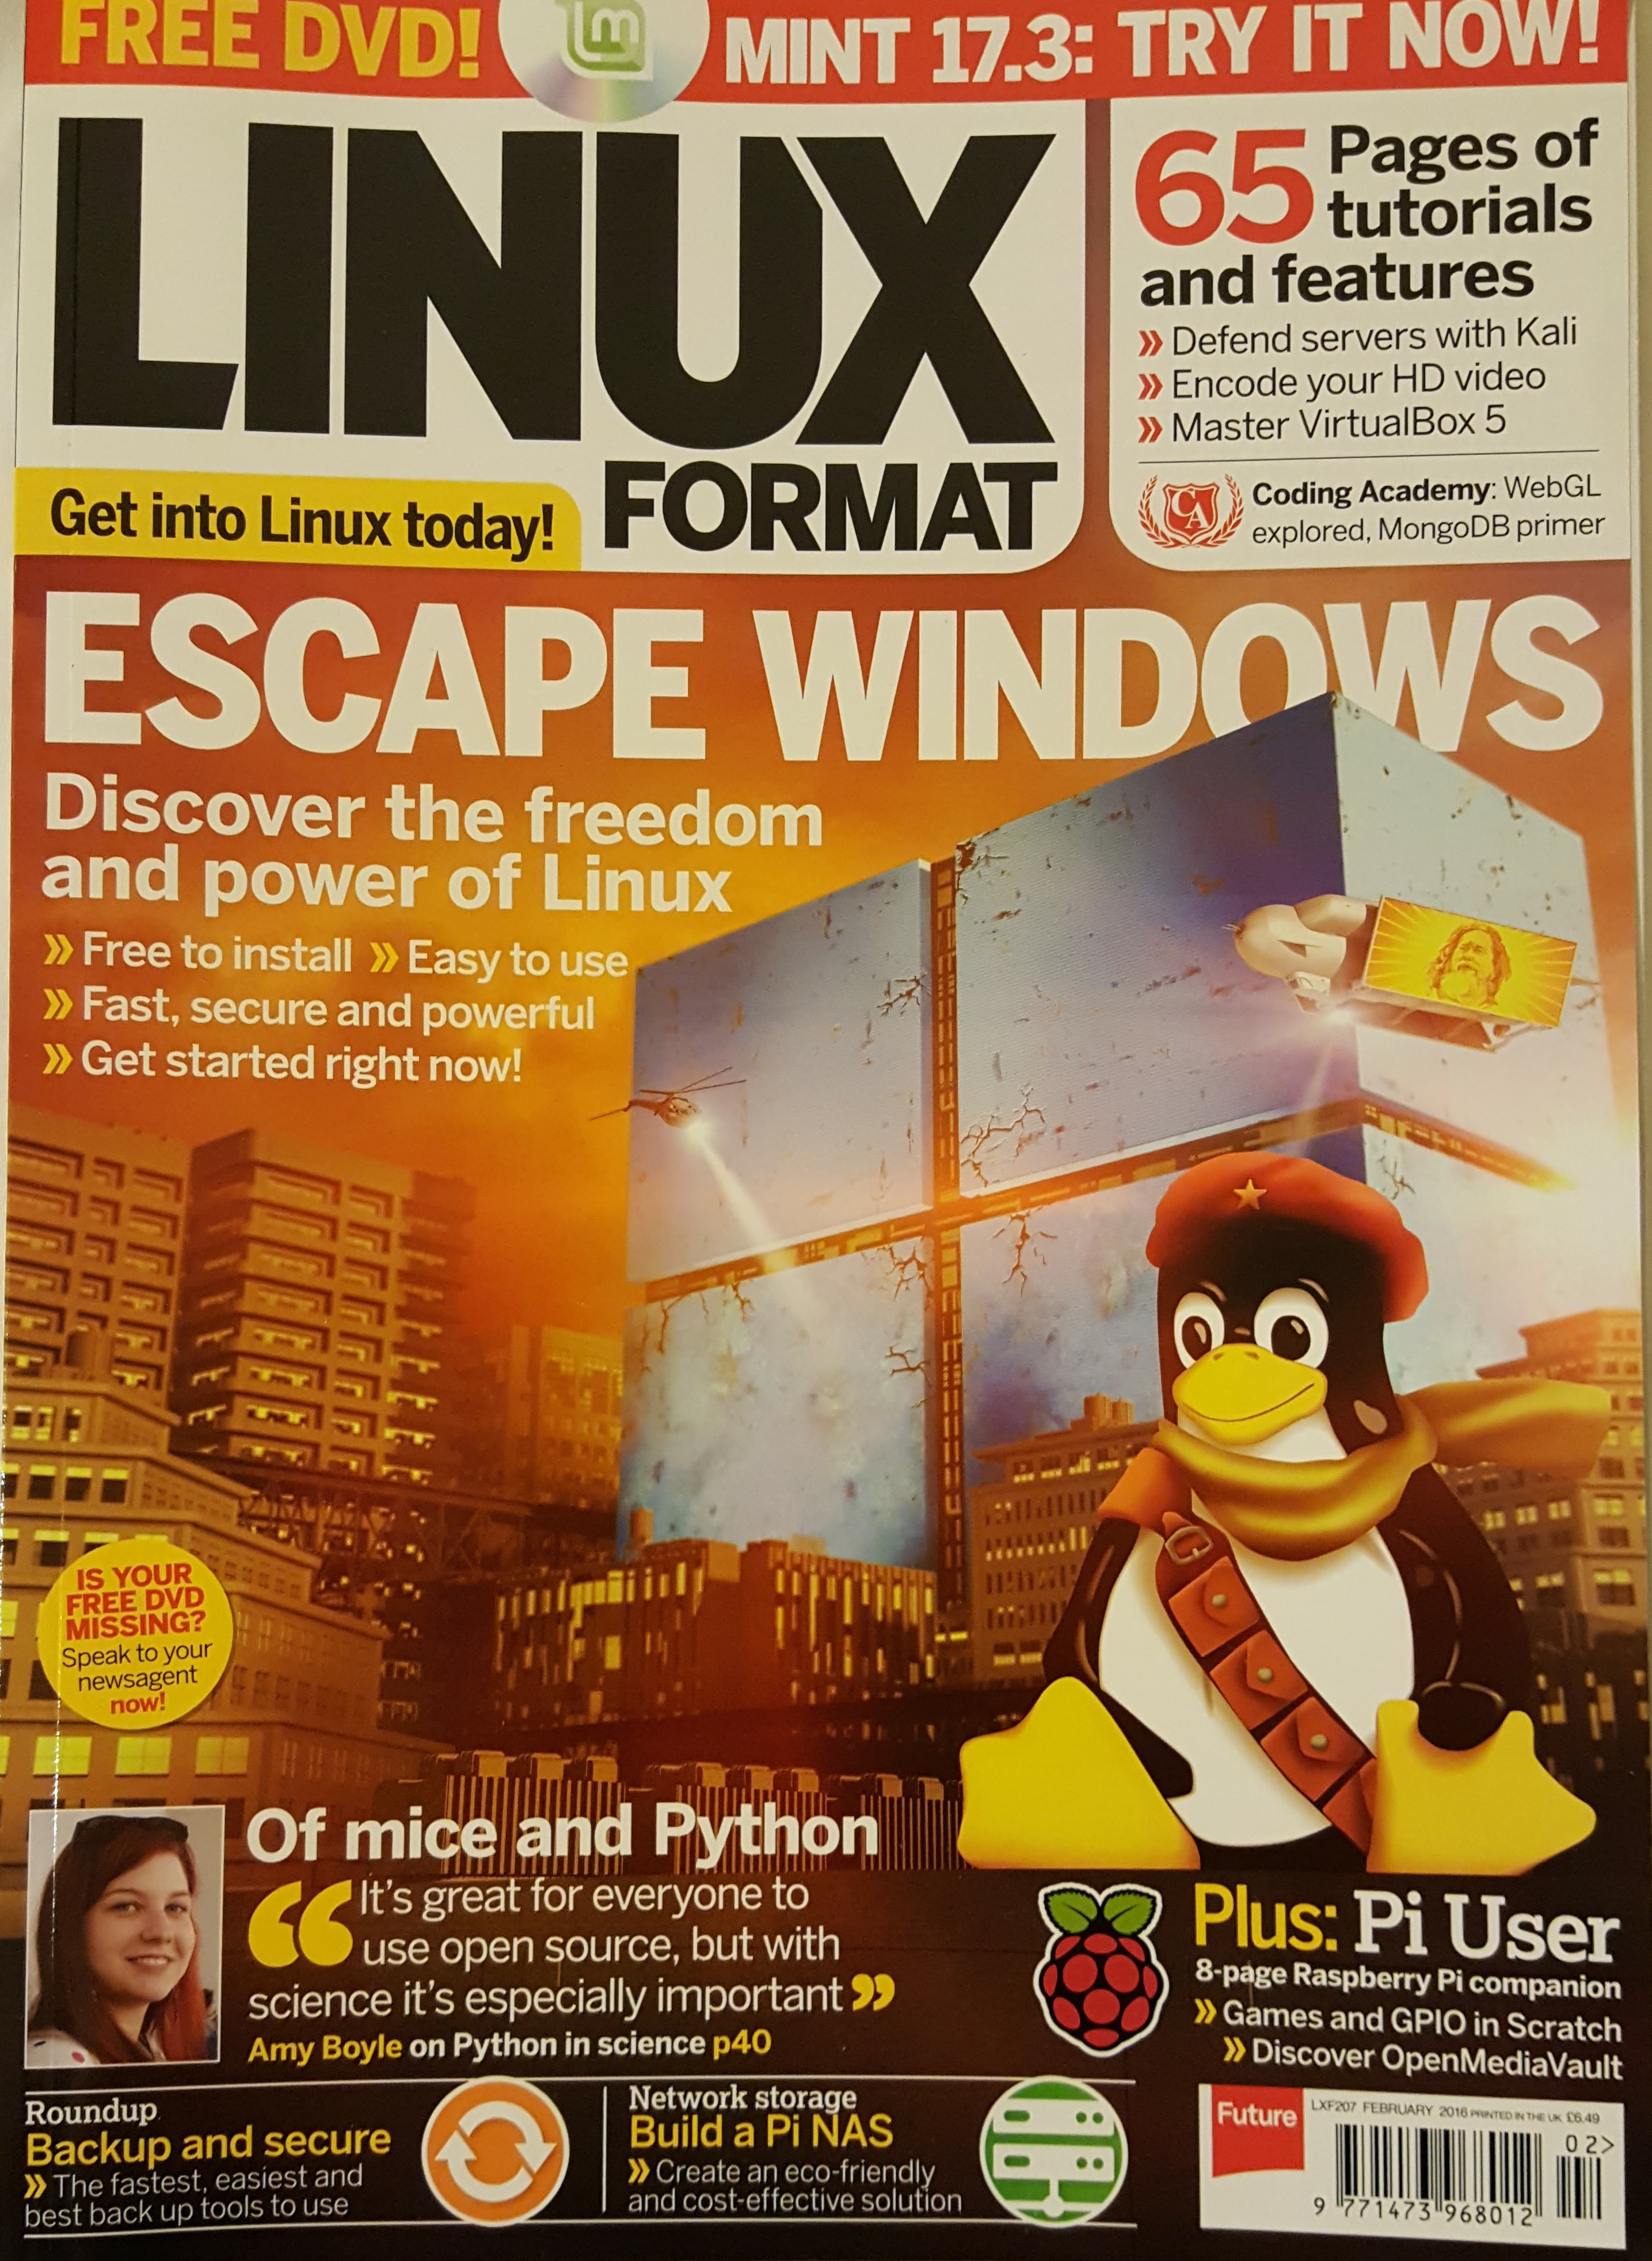
\includegraphics[width=.8\textwidth]{./images/LF-201602}
        		\end{figure}
	\end{columns}
	\end{frame}








	\begin{frame}
	\frametitle{}
	\framesubtitle{}
	\centering\huge
	Feel Free\\
	Be Free!
	\end{frame}


\end{document}

